\section{Flag 12 - Recover}

\paragraph{1D4855F7337C0C14B6F44946872C4EB33853F40B2D54393FBE94F49F1E19BBB0}
\begin{center}
    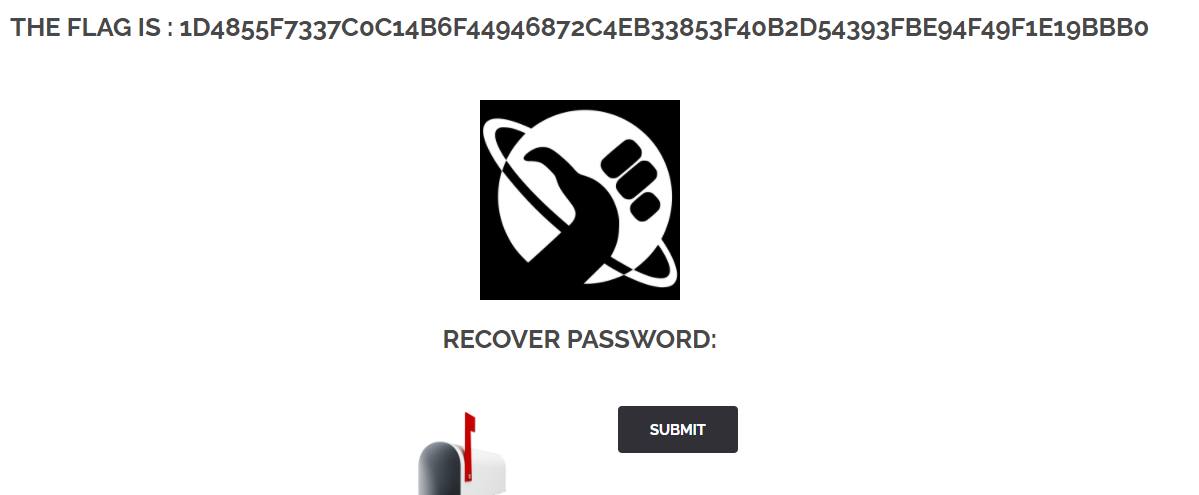
\includegraphics[width=0.5\textwidth]{15.Flag12/12-07.png}\\[0cm] 
\end{center}

\subsection{Vulnerability}

A poorly designed password recovery page. It is susceptible to compromise meaning one could login in easily and steal information or retrieve which emails have active accounts.

\subsection{Location}

`http://<ip-address>:80/?page=recover`

\subsection{Method}

The page shows only a Submit button and a mailbox. When you inspect the code you will see a few things but mainly:

```

<form action="\#" method="POST">

    <input type="hidden" name="mail" value="webmaster@borntosec.com" maxlength="15">
  
    <input type="submit" name="Submit" value= "Submit">

</form>

```

If you change the type from hidden to text, it will appear on your screen. Ideally a fix would be changing it to email. The content already has a value set rather than a placeholder. Changing the value and submitting results in the flag being returned.

The other issue is that there is a limit of 15 characters which is small and makes it easier to guess when one subtracts an email suffix i.e @gmail.com, @hotmail.com or @borntosec.co.za

\subsection{Tools}

\begin{figure}[!htb]
    \centering
    \subfloat[Login Page]{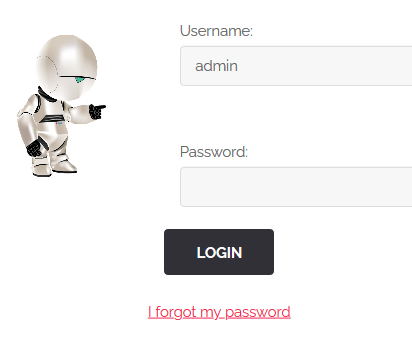
\includegraphics[width=.45\columnwidth]{15.Flag12/12-01.png}\label{fig: 12-01 - wtf}} \quad
    \subfloat[Recovery page]{
\includegraphics[width=.45\columnwidth]{15.Flag12/12-02.png}\label{fig: 12-02 - wrong}} \\
    \subfloat[Inspect code]{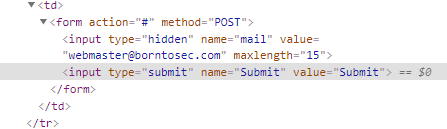
\includegraphics[width=.45\columnwidth]{15.Flag12/12-03.png}\label{fig: 12-03 - wtf}} \quad
    \subfloat[Hidden Agendas]{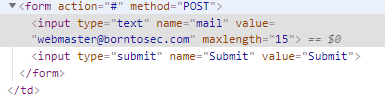
\includegraphics[width=.45\columnwidth]{15.Flag12/12-04.png}\label{fig: 12-04 - wrong}} \\
    \subfloat[Recover the password]{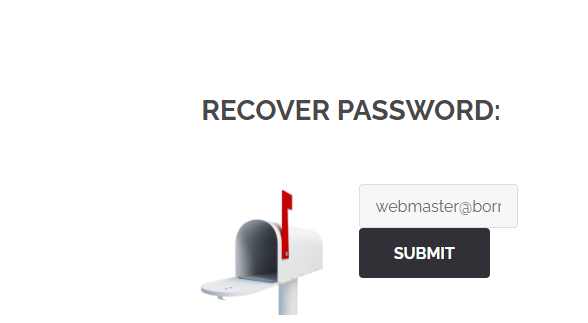
\includegraphics[width=.45\columnwidth]{15.Flag12/12-05.png}\label{fig: 12-05 - wtf}} \quad
    \subfloat[Change email address]{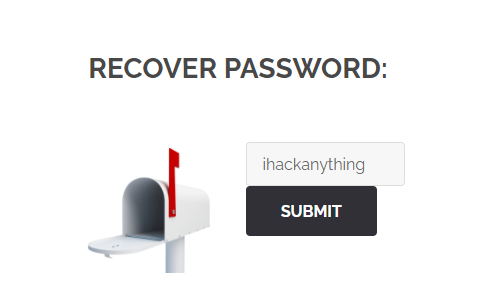
\includegraphics[width=.45\columnwidth]{15.Flag12/12-06.png}\label{fig: 12-06 - wrong}} \\
    \caption[Flag 12 Method]{Process to Capture the Recover Flag} % The text in the square bracket is the caption for the list of figures while the text in the curly brackets is the figure caption
    \label{fig:flag12 method}
\end{figure}

\begin{itemize}
    \item \href{https://cheatsheetseries.owasp.org/cheatsheets/Forgot_Password_Cheat_Sheet.html}{OWASP}
    \item \href{https://www.trustwave.com/en-us/resources/blogs/spiderlabs-blog/exploiting-password-recovery-functionalities/}{TrustWave}
\end{itemize}

\subsection{Remedy}

\begin{itemize}
    \item Return a consistent message for both existent and non-existent accounts.
    \item Ensure that the time taken for the user response message is uniform.
    \item Use a side-channel to communicate the method to reset their password.
    \item Use URL tokens for the simplest and fastest implementation.
    \item Ensure that generated tokens or codes are:
        \subitem Randomly genererated using a cryptographically safe algorithm.
        \subitem Sufficiently long to protect against brute-force attacks.
        \subitem Stored securely.
        \subitem Single use and expire after an appropriate period.
    
    It is also important to use a placeholder rather than a value. Ensure that there is a validator to make sure it is a valid email, provide standard feedback regardless of whether the recovery was successful or not.
    
    Return a link and not the actual password, or use two-factor authentication.
    
\end{itemize}